\large Team:
\large  Introduction
	\begin{figure}[H]
		introduction\\
		\emph{Team PML 30 ϕ was assembled in September 2014 from 3 novices and one participant with experience as a captain. Among the participants were assigned tasks and roles, 			set safety rules. In the first place in the team was put noble professional spread it to the masses.  All decisions taken collectively in team with discussion and finding optimal 			 	solutions. 
		During the year we took part in many events and anywhere we have tried attract our team and to encourage people to take part in FTC. Also everywhere pursuing and 				distribution the principles of noble professional. Talk to the press, we would like attract more attention to our team and to the competition in general, as well as attracting 				sponsors. The last was important because of the need for funds for the purchase of materials and equipment that cost really a lot.
		Team took part in the three qualifying competitions and the regional finals. In all of them make new contacts, share experience and provide mutual assistance with other teams. 
		In the first qualifying rounds in Sochi we have contacts Stuy  fission 310 team from USA, and maintain contact with them to this day. On regional finals, we met with a team from 			Romania Auto Vortex keep in touch by Facebook. Also, there is an active dialogue with a large number of Russian teams. Team page in Facebook you can find the desired address 			https://www.facebook.com/pages/FTC-team-PML30-PHI.
}
 
\end{figure}
\begin{figure}[H]
	\begin{minipage}[h]{0.47\linewidth}
		\center{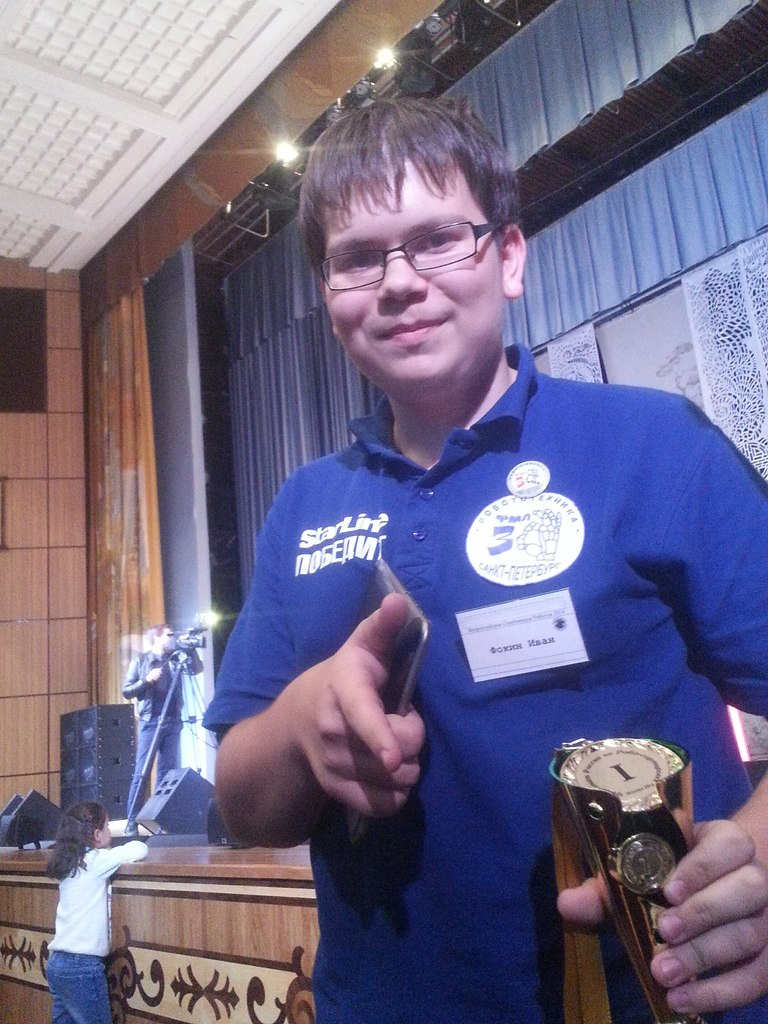
\includegraphics[scale=0.2]{days/Team/images/01}}\\
		Fokin Ivan\\
		\emph{Part in the command: captain,   purchase of materials,  development strategy in the game,  communication with the press, reserve  manipulator }
		\emph{Information: 17 years old, in robotics 5 years, in FTC 3 years } 
	\end{minipage}
	\hfill
	\begin{minipage}[h]{0.47\linewidth}
		\center{
\includegraphics[scale=0.25]{days/Team/images/02}}\\
		Radionov Maxim\\
		\emph{Part in the command: communication with the team and community, decorating robot, Power Design, reserve operator  }
		\emph{Information: 17 years old, in robotics 3 years, in FTC 1 years}
	\end{minipage}
	\center  
	\center  
	\vfill 
	\begin{minipage}[h]{0.47\linewidth}
		\center{
\includegraphics[scale=0.25]{days/Team/images/03}}\\
		Safronov Nikita\\
		\emph{Part in the command: manipulator-1,  creation of 3D models, chief engineer, responsible for the assembly robot}
		\emph{Information: 16 years old, in robotics 3 years, in FTC 1 years} 
	\end{minipage}
	\hfill
	\begin{minipage}[h]{0.47\linewidth}
		\center{
\includegraphics[scale=0.25]{days/Team/images/04}}\\
		Maksimychev Evgenuy\\
		\emph{Part in the command: manipulator-2, responsible for the technic of safety, responsible for the writting of technical book}
		\emph{Information: 15 years old, in robotics 2 years, in FTC 1 years}
	\end{minipage}
\end{figure}

\newpage

\large  Instructors:

\begin{figure}[H]
	\begin{minipage}[h]{0.47\linewidth}
		\center{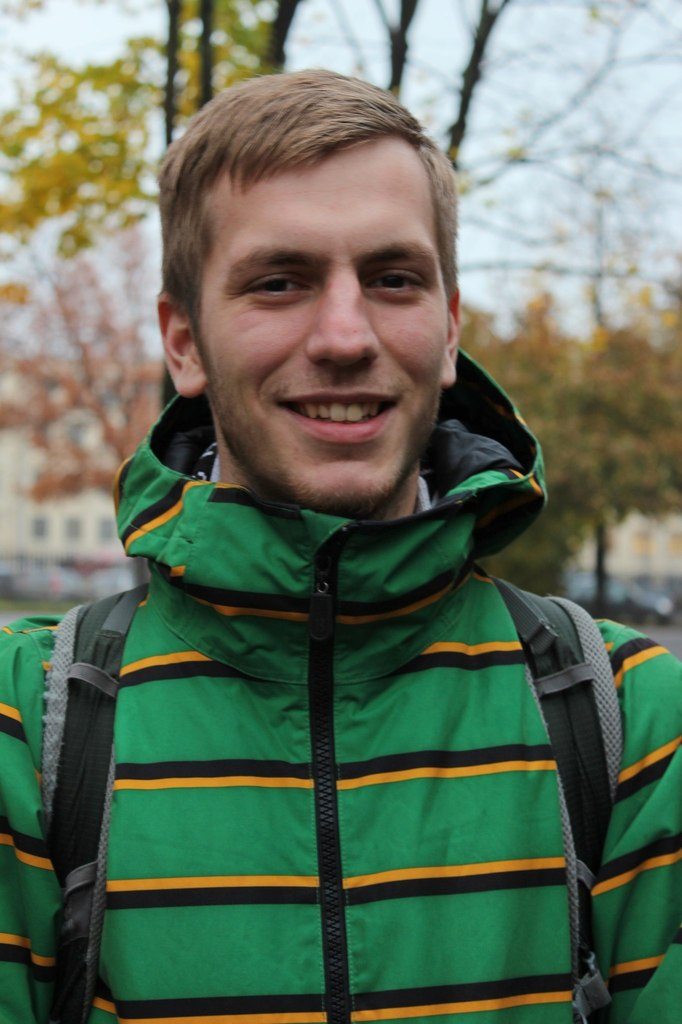
\includegraphics[scale=0.25]{days/Team/images/05}}\\
		\emph{Fedotov Anton} 
	\end{minipage}
	\hfill
	\begin{minipage}[h]{0.47\linewidth}
		\center{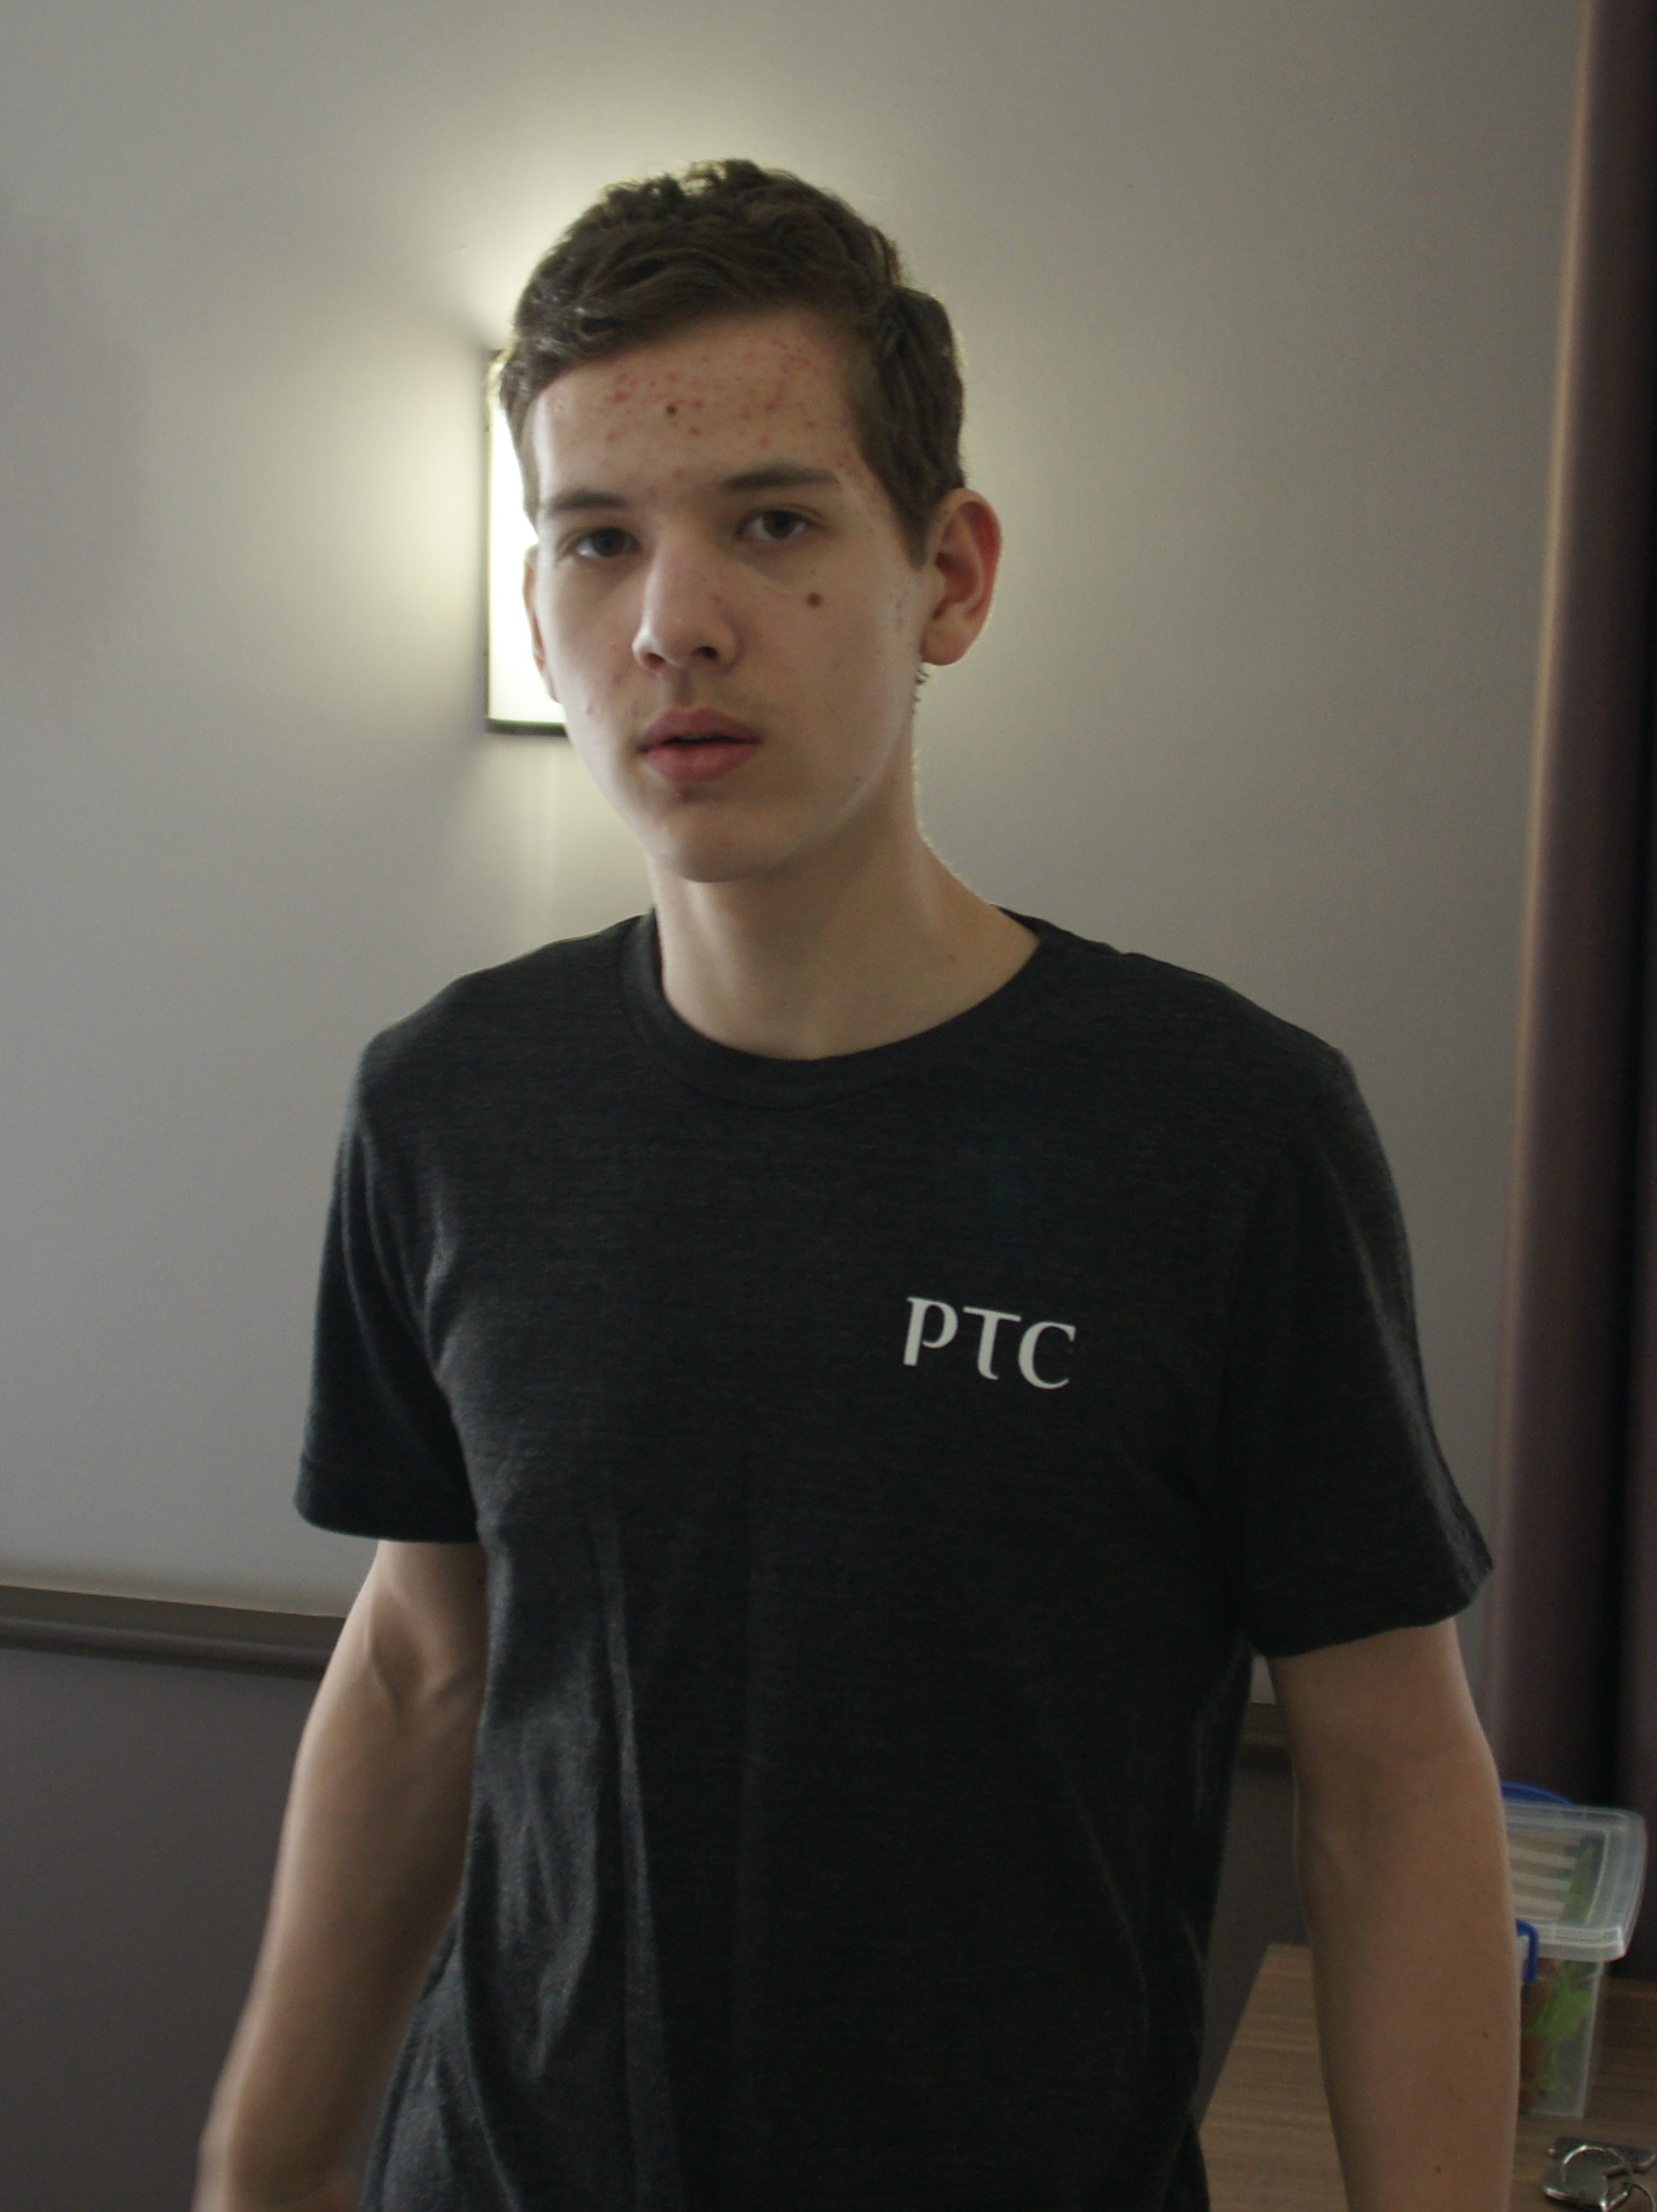
\includegraphics[scale=0.12]{days/Team/images/06}}\\
		\emph{Krylov Georguy}
	\end{minipage}
	\center  
	\center  
	\vfill 
	\begin{minipage}[h]{0.47\linewidth}
		\center{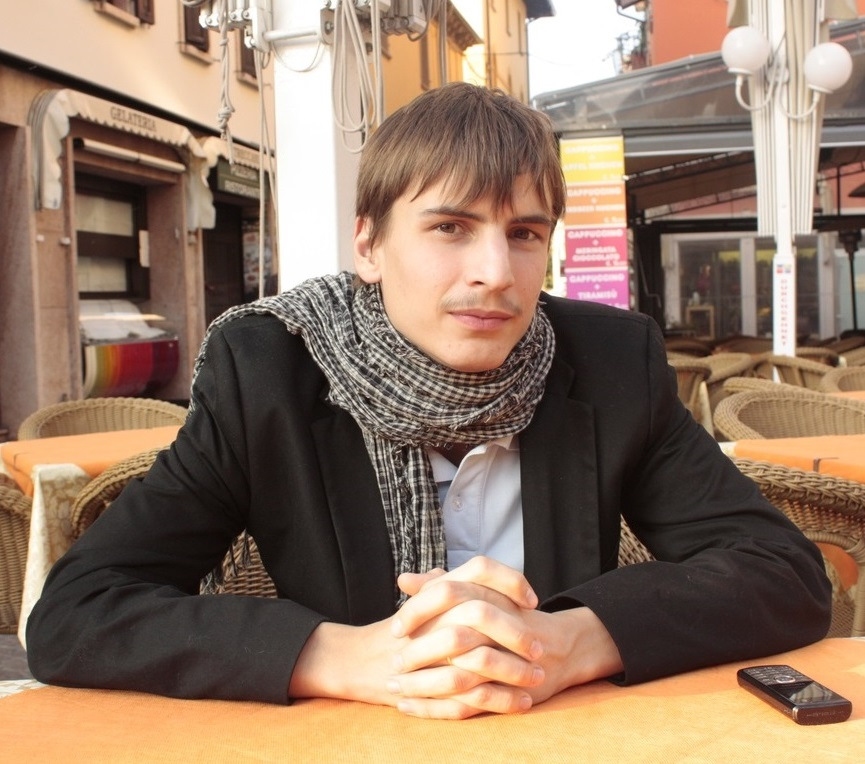
\includegraphics[scale=0.3]{days/Team/images/07}}\\
		\emph{Luzin Dmitruy}
	\end{minipage}
	\hfill
	\begin{minipage}[h]{0.47\linewidth}
		\center{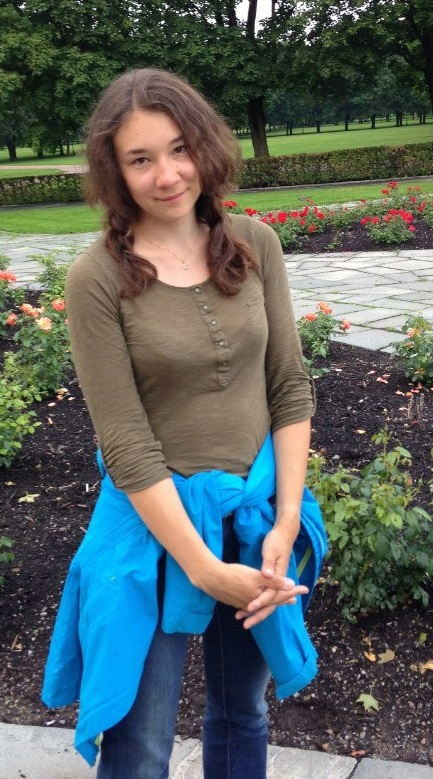
\includegraphics[scale=0.35]{days/Team/images/08}}\\
		\emph{Luzina Kate}
	\end{minipage}
\end{figure}

\newpage
